\documentclass{article}

\usepackage{biblatex}
\addbibresource{sources.bib}

\usepackage{csquotes}

\usepackage{graphicx}

\usepackage{multicol}

\title{Rapport - IPASS}
\author{Jimmy Bierenbroodspot}
\date{26 juni 2024}

\begin{document}
\begin{titlepage}
    \maketitle
\end{titlepage}

\section{Probleembeschrijving}

In de toekomst willen wij graag een AI-model hebben, dat de beste CV's op de
markt kan maken voor onze klanten. Hiervoor hebben we natuurlijk veel data in de
vorm van CV's nodig en gelukkig hebben we deze in grote aantallen. Nu is het
probleem dat deze CV's in .pdf-formaat opgeslagen zijn en text hieruit halen is
niet makkelijk \cite{timalsina-2024}.

We hebben het programma genaamd PyPDF\cite{unknown-author-2024} waarmee we in
staat zijn om text uit .pdf-bestanden te lezen, het probleem is dat dit
ongestructureerd is. Als voorbeeld kunnen we het voorbeeld CV in \ref{fig:cv-example}
nemen.

\begin{figure}[ht]
    \begin{center}
        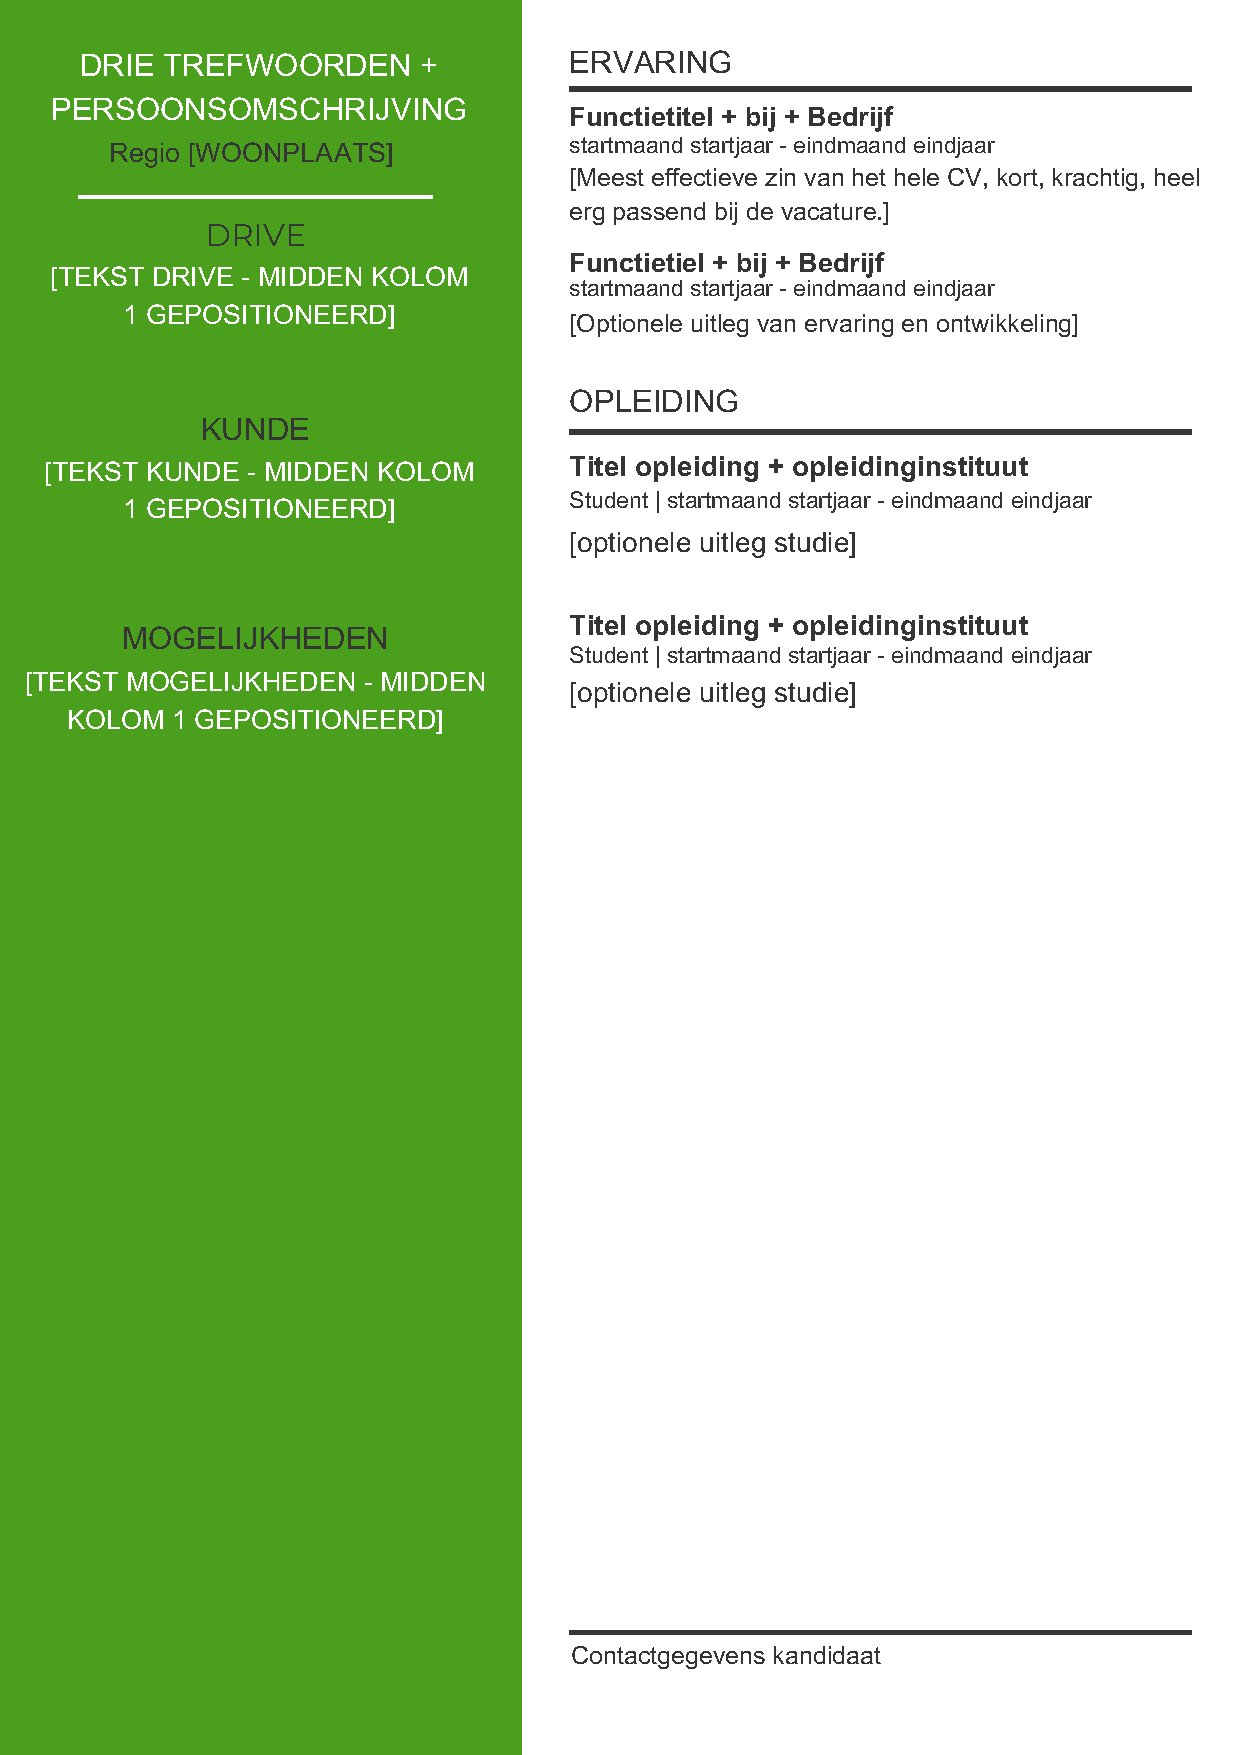
\includegraphics[width=0.5\linewidth]{pdf/voorbeeld_aicv_cv.pdf}
    \end{center}
    \caption{Voorbeeld van een Cliq CV}
    \label{fig:cv-example}
\end{figure}

In \ref{fig:pypdf-no-layout} kunnen we zien wat er gebeurd als we de tekst
uit \ref{fig:cv-example} lezen. Dit ziet er uit als een onlogisch rommeltje.
We kunnen met PyPDF echter ook de tekstopmaak kopiëren, zoals te zien in
\ref{fig:pypdf-w-layout}. Dit ziet er al beter uit maar als we bedenken dat
dit allemaal op een regel staat, waarbij de nieuwe regels in dit geval juist
worden getoond, maar eigenlijk aangeduid wordt met een \textbackslash n.

\begin{figure}[ht]
    \begin{center}
        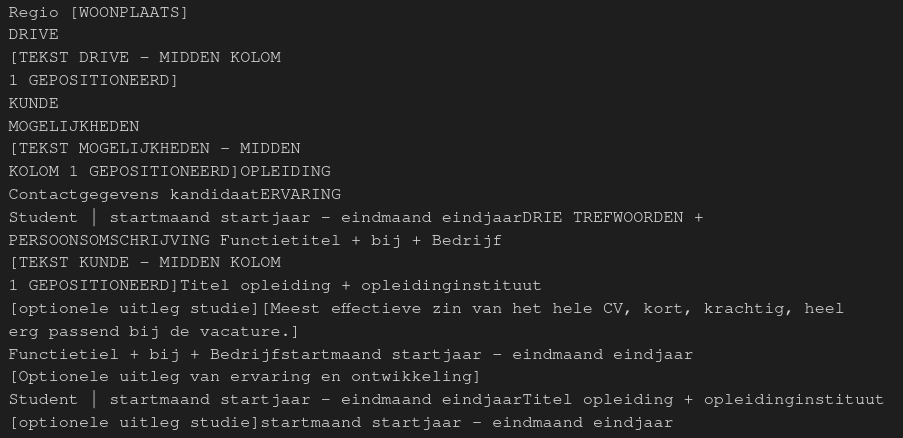
\includegraphics[width=\linewidth]{img/voorbeeld_pypdf_text_extract_geen_layout.png}
    \end{center}
    \caption{Voorbeeld van tekstextractie PyPDF}
    \label{fig:pypdf-no-layout}
\end{figure}

\begin{figure}[ht]
    \begin{center}
        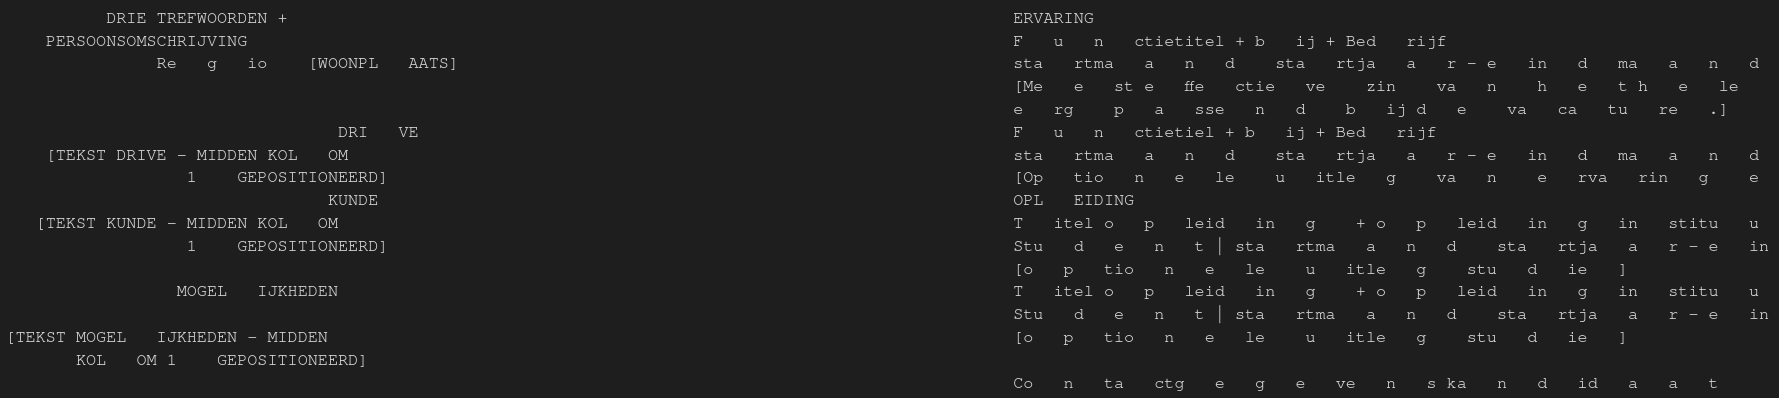
\includegraphics[width=\linewidth]{img/voorbeeld_pypdf_text_extract_layout.png}
    \end{center}
    \caption{Voorbeeld van tekstextractie PyPDF met tekstopmaak}
    \label{fig:pypdf-w-layout}
\end{figure}

\vfill

\subsection{Waarom willen we dit?}

In datawetenschap kennen we het concept GIGO, oftewel garbage in garbage out
\cite{merriam-webster-no-date}. Als we aannemen dat ditzelfde zal gelden voor
het model dat we gaan gebruiken dan zouden we graag willen dat onze invoerdata
gestructureerd is.

Als we aannemen dat de tekst op een regel zou moeten komen te staan om ingelezen
te worden door het model, dan zijn beide manieren van text extraheren met PyPDF
niet gestructureerd. We willen dus dat de tekst op een logische volgorde komt te
staan. Als een CV geen kolommen zou bevatten dan kunnen we met PyPDF de
tekstopmaak kopiëren, nu weten we alleen van tevoren niet of een CV kolommen
heeft of niet en als dat wel zo is weten we niet hoeveel kolommen er zijn. Om
hierachter te komen moeten we naar het CV kijken en dat gaat niet met een
geautomatiseerd proces.

\section{Eisen}

De opdrachtgever heeft in ieder geval de volgende eisen gegeven:

\begin{enumerate}
    \item Er moet een CV bestand ingelezen worden.
    \item Het aantal kolommen moet teruggegeven worden.
\end{enumerate}

Verder zijn er geen functionele of prestatie-eisen.

\section{Algoritme}

In \ref{fig:pypdf-w-layout} kunnen we zien dat er een best duidelijke scheiding
zit tussen de twee kolommen. We hebben besloten om hier Lloyds algoritme
(zie\cite{lloyd-1982}) voor te gebruiken omdat het een makkelijke en snelle
oplossing leek te zijn voor dit probleem.

Om erachter te komen hoeveel kolommen het optimale aantal zou zijn gebruiken we
de elleboog methode, deze werkt als volgt\cite{ropensci-no-date}:

\begin{enumerate}
    \item Voor elk gewilde aantal clusters wordt het model getraind.
    \item Elke keer dat het model getraind is wordt de error opgeslagen.
    \item Er wordt een rechte lijn van de eerste observatie naar de laatste
          observatie getrokken.
    \item Bereken de afstand tussen deze lijn en elke score.
    \item Neem het aantal clusters van de score die het verst van deze lijn
          verwijderd is.
\end{enumerate}

\section{Resultaat}

Na het evalueren van het model op een dataset van 116 bestaande CV's zien we een
teleurstellend resultaat. We weten maar van ongeveer 15\% van de gevallen het
juiste aantal kolommen te vinden. Dit is echt veel te weinig om in een
productieomgeving te gebruiken.

\section{In het vervolg}

We zouden in de toekomst willen kijken of de volgende verbeterpunten het
presteren van de clusteringsaanpak zal vergroten:

\begin{itemize}
    \item het model meerdere keren uitvoeren met verschillende willekeurige
          clustercentra voor elke keer dat het model getraind wordt.
    \item Kmeans++ gebruiken.
    \item De invoerdata standaardiseren.
\end{itemize}

Ook zouden we dit probleem graag als classificatieprobleem willen proberen
aanpakken aangezien dit daadwerkelijk ondersteund wordt door bestaande
literatuur.

\printbibliography

\listoffigures

\listoftables

\end{document}